\documentclass[11pt,letterpaper]{article}

\usepackage[margin=1in]{geometry}
\usepackage[T1]{fontenc}
\usepackage{lmodern}
\usepackage{microtype}
\usepackage{booktabs}
\usepackage{array}
\usepackage{graphicx}
\usepackage{tikz}
\usetikzlibrary{positioning,arrows.meta}
\usepackage{pgf}
\usepackage[hidelinks]{hyperref}
\usepackage{fancyhdr}
\usepackage{listings}

% ---- Project metadata (edit here) -------------------------------------
\newcommand{\projecttitle}{Densor}
\newcommand{\projectsubtitle}{Sensor Density and Building Inference}
\newcommand{\authorname}{Jake Lambert}
\newcommand{\institution}{[Institution]}
\newcommand{\program}{Master of Science in Data Science}
\newcommand{\advisor}{[Advisor]}
\newcommand{\projectterm}{Capstone Project, 2026--2027}
% -----------------------------------------------------------------------

\pagestyle{fancy}
\fancyhf{}
\renewcommand{\headrulewidth}{0pt}
\fancyfoot[C]{\thepage}

\lstset{basicstyle=\ttfamily\small,breaklines=true,frame=single,columns=fullflexible}

\newcommand{\todo}[1]{\textbf{[TODO: #1]}}

% Cost table rows: \costrow{item}{qty}{unit price in USD, 0 = not yet entered}
\newcounter{costrows}
\newcommand{\hwtotal}{0}
\newcommand{\costrow}[3]{%
  \pgfmathsetmacro{\linetotal}{#2*#3}\xdef\linetotal{\linetotal}%
  \pgfmathsetmacro{\hwtotal}{\hwtotal+\linetotal}%
  \xdef\hwtotal{\hwtotal}%
  #1 & #2 & \ifdim #3pt=0pt TBD\else\$\pgfmathprintnumber[fixed,zerofill,precision=2]{#3}\fi
     & \ifdim #3pt=0pt TBD\else\$\pgfmathprintnumber[fixed,zerofill,precision=2]{\linetotal}\fi \\
}

\begin{document}

% ========================= Cover page ====================================
\begin{titlepage}
  \centering
  \vspace*{1.2in}
  {\Huge\bfseries \projecttitle\par}
  \vspace{0.4cm}
  {\Large \projectsubtitle\par}
  \vspace{1.5cm}
  {\large Does increasing sensor density yield step increases in\\
  the inferences we can make about a home?\par}
  \vfill
  {\large \authorname\par}
  \vspace{0.3cm}
  \program\\
  \institution\par
  \vspace{0.3cm}
  Advisor: \advisor\par
  \vspace{0.3cm}
  \projectterm\par
  \vspace{0.3cm}
  \textit{Working draft, \today}\par
  \vspace{0.8in}
\end{titlepage}

\tableofcontents
\clearpage

% ========================= Introduction ==================================
\section{Introduction}
\todo{Motivation, thesis, and research questions. Draft thesis: increasing
sensor density yields step increases in the inferences available about a home
or building, with diminishing returns. This is a work in progress.}

The hypothesis is tested by ablation: the same recorded dataset is analyzed using
1, 2, 5, 10, and $N$ sensors, and the inferences available at each density are
compared. Thermostat API integration and a recommendations engine are out of
scope.

Project code is kept in a repository at
\url{https://github.com/djake/densor}.

% ========================= Initial configuration =========================
\section{Initial Configuration}
\label{sec:initial-config}

The proof of concept (fall semester 2026) starts with two sensors and a single
low-power host. This configuration is intentionally minimal: it exercises the
whole data path end to end before the deployment is scaled to 10 or more
sensors per household.

\subsection{Hardware}

\begin{itemize}
  \item \textbf{Sensors:} two Sonoff SNZB-02P Zigbee temperature and humidity
    sensors, battery powered. They are named \texttt{densor-ch-01} and
    \texttt{densor-ch-02} (``ch'' denotes the house).
  \item \textbf{Coordinator:} Sonoff Zigbee 3.0 USB Dongle Plus MG24.
  \item \textbf{Host:} Raspberry Pi 3 B+ (1\,GB RAM), running Raspberry Pi OS
    Lite (64-bit), headless. The hostname and user are \texttt{densor}.
\end{itemize}

\subsection{Software and data path}

Zigbee2MQTT bridges the Zigbee network to an MQTT broker (Mosquitto). A Python
logger subscribes to the sensor topics and writes each reading to a SQLite
database on the Pi, which is the source of truth. A separate hourly job exports
each closed hour as a Parquet file and uploads it to an S3-compatible bucket
(Tigris) for analysis. Zigbee2MQTT and Mosquitto are enabled at boot under
systemd, as are the logger and the upload timer.

\begin{figure}[ht]
\centering
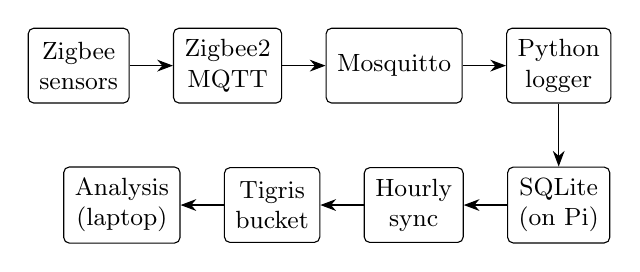
\begin{tikzpicture}[
  node distance=0.55cm and 0.55cm,
  box/.style={draw,rounded corners=2pt,align=center,minimum height=0.95cm,
              inner sep=4pt,font=\small},
  arr/.style={-{Stealth[length=2mm]}}]
  \node[box] (s)  {Zigbee\\sensors};
  \node[box,right=of s]  (z) {Zigbee2\\MQTT};
  \node[box,right=of z]  (m) {Mosquitto};
  \node[box,right=of m]  (l) {Python\\logger};
  \node[box,below=0.8cm of l] (db) {SQLite\\(on Pi)};
  \node[box,left=of db]  (sy) {Hourly\\sync};
  \node[box,left=of sy]  (b) {Tigris\\bucket};
  \node[box,left=of b]   (a) {Analysis\\(laptop)};
  \draw[arr] (s)--(z); \draw[arr] (z)--(m); \draw[arr] (m)--(l);
  \draw[arr] (l)--(db); \draw[arr] (db)--(sy); \draw[arr] (sy)--(b);
  \draw[arr] (b)--(a);
\end{tikzpicture}
\caption{Data path of the initial two-sensor configuration.}
\label{fig:datapath}
\end{figure}

\subsection{Key configuration choices}

\begin{itemize}
  \item \textbf{Zigbee channel:} 25.
  \item \textbf{Device identity:} readings are keyed on each sensor's permanent
    IEEE address; the friendly name is stored as metadata and can change without
    breaking the record.
  \item \textbf{Timestamps:} assigned on arrival at the Pi, in UTC. Sensors
    report in $^\circ$C.
  \item \textbf{Collection frequency:} working target of one reading per
    minute per sensor.
  \item \textbf{Cloud layout:} immutable per-hour Parquet objects at
    \texttt{readings/date=\allowbreak YYYY-MM-DD/\allowbreak hour=HH.parquet}, plus a
    \texttt{devices.json} mapping. Object stores have no append operation, so
    each hour is written once after it closes. If the Pi is offline, local
    collection continues and missed hours upload on the next run.
  \item \textbf{Remote access:} ZeroTier private network with no port
    forwarding; SSH using an Ed25519 key held in 1Password, with password
    authentication disabled on the Pi.
\end{itemize}

\subsection{Power-outage assumptions}

No readings are collected during an outage. The Pi reboots on its own when power
returns and all services restart. SD-card corruption risk is mitigated by a
high-endurance card and small, frequent database commits. \todo{Verify with a
reboot test and a pull-the-plug test, and record results.}

\subsection{Status}

The logger and upload code have been tested locally only. \todo{Deploy to the
Pi, then record first-week observations: reporting interval versus battery,
sensor-to-sensor offsets, and firmware consistency.}

% ========================= Cost summary ==================================
\subsection{Cost Summary}
\label{sec:cost}

Table~\ref{tab:cost} lists the cost of the initial two-sensor configuration.
The sensors were bought in an Amazon order on October 5, 2026, and the Pi kit,
coordinator dongle, and microSD card in a second Amazon order on October 9, 2026.
Tax is the sum of the two orders. To change a price, edit the third argument of the
corresponding \verb|\costrow| in the source and totals update automatically.

\begin{table}[ht]
\centering
\caption{Hardware cost of the initial configuration (USD).}
\label{tab:cost}
\begin{tabular}{@{}lrrr@{}}
\toprule
Item & Qty & Unit & Total \\
\midrule
\costrow{CanaKit Raspberry Pi 3 B+ kit (Pi, clear case, 2.5\,A power supply)}{1}{89.99}
\costrow{Sonoff Zigbee 3.0 USB Dongle Plus MG24 (coordinator)}{1}{35.90}
\costrow{SanDisk MAX Endurance 32\,GB microSDHC card}{1}{35.99}
\costrow{Sonoff SNZB-02P temperature/humidity sensor, 2-pack}{1}{29.90}
\costrow{Sales tax (Amazon orders of Oct.\ 5 and Oct.\ 9, 2026)}{1}{11.58}
\midrule
\multicolumn{3}{@{}l}{Hardware subtotal} &
  \ifdim \hwtotal pt=0pt TBD\else\$\pgfmathprintnumber[fixed,zerofill,precision=2]{\hwtotal}\fi \\
\bottomrule
\end{tabular}
\end{table}
\xdef\firsttotal{\hwtotal}

\paragraph{Recurring and software costs.}
Zigbee2MQTT, Mosquitto, ZeroTier (free tier), and the Python libraries used are
free. Cloud storage on Tigris is billed by usage; at the expected data volume
(a few readings per minute per sensor) it should be small. \todo{Record the
actual Tigris charges once the bucket is in use.}

\paragraph{Marginal cost per sensor.}
Because the Pi, dongle, and storage are fixed costs, scaling the deployment adds
only the SNZB-02P unit price per sensor (\$14.95 each in the 2-pack, before tax). This is the figure that matters for the
10--100 sensor target and is reported in the final analysis.


% ========================= POC round 2 ===================================
\section{Proof of Concept, Round 2}
\label{sec:poc2}

\subsection{Goals}

The primary goal of round 2 is to configure the system to use a lower-cost
sensor, and to add sensor types beyond indoor temperature and humidity.
Specifically:
\begin{enumerate}
  \item \textbf{Lower-cost sensor.} Test the Sonoff SNZB-02B against the
    SNZB-02P used in round 1, to see whether it can be the standard sensor when
    scaling to 10 or more sensors per household.
  \item \textbf{Outdoor reference.} Add an outdoor temperature and humidity
    sensor at each site, to replace or supplement public weather data with
    values measured at the building.
  \item \textbf{Air pressure.} Add an indoor air-pressure sensor at each site,
    to compare against outdoor pressure as an indicator of infiltration.
  \item \textbf{Second site.} Instrument a second house with the same data
    path, so that results can be compared across two buildings.
\end{enumerate}

\subsection{Hardware}

Table~\ref{tab:round2-hw} lists the round-2 hardware. The second Raspberry Pi
kit and Zigbee dongle form the host for the second site. The outdoor and
pressure sensors are split between the two sites, one of each per site. The
SNZB-02B 4-pack is for the sensor comparison.

\begin{table}[ht]
\centering
\caption{Round-2 hardware and its use.}
\label{tab:round2-hw}
\begin{tabular}{@{}p{2.6in}rp{2.4in}@{}}
\toprule
Item & Qty & Use \\
\midrule
Sonoff SNZB-02B (AirGuard TH Lite), 4-pack & 1 & Lower-cost indoor sensor, compared against the SNZB-02P \\
Sonoff SNZB-02WD (IP65, LCD) & 2 & Outdoor temperature and humidity, one per site \\
Sonoff SNZB-02M (AirGuard TH Pressure) & 2 & Indoor temperature, humidity, and air pressure, one per site \\
CanaKit Raspberry Pi 3 B+ kit & 1 & Host for the second site \\
Sonoff Zigbee 3.0 USB Dongle Plus MG24 & 1 & Zigbee coordinator for the second site \\
\bottomrule
\end{tabular}
\end{table}

Per the manufacturers' published specifications, the outdoor SNZB-02WD is rated
IP65 and to $-20^\circ$C, with $\pm0.5^\circ$C and $\pm3\%$ RH accuracy and a
CR2477 coin cell. The SNZB-02M reports temperature ($\pm0.2^\circ$C), humidity
($\pm2\%$ RH), and pressure ($\pm0.1$\,hPa). The SNZB-02B has the same
temperature and humidity accuracy as the SNZB-02P, runs on two AAA cells, and
has no display. The Zigbee2MQTT device pages list all three as supported. The
SNZB-02WD exposes battery, voltage, temperature, humidity, and calibration
offsets; the SNZB-02M adds pressure and calibration for temperature, humidity,
and pressure.

\subsection{Sensor comparison: SNZB-02B against SNZB-02P}
\label{sec:sensor-comparison}

At about \$14.95 per sensor, the SNZB-02P sets a floor on the cost of scaling to
10 to 100 sensors. The SNZB-02B costs about \$8.98 each in the 4-pack
(\$35.90), roughly 40\% less. Its reporting interval and battery life at one
reading per minute are not yet known. The manufacturer's product overview is at
\url{https://help.sonoff.tech/docs/SNZB02B}.

\textbf{Test design.} Place the two SNZB-02P sensors and the four SNZB-02B
sensors together in one location for about a week, on the same Zigbee network
and logging path. Compare:
\begin{itemize}
  \item mean offset of each sensor from the group mean (relative only, since no
    reference thermometer is available);
  \item noise, as the standard deviation of each sensor's difference from the
    group mean;
  \item reporting interval distribution, and gaps in the record;
  \item battery level over the week, and link quality.
\end{itemize}

\textbf{Decision rule.} Adopt the SNZB-02B for scaling if its offsets are stable
enough to remove with the built-in calibration setting, it reports about once a
minute without gaps, and its battery drain projects to a usable life.
Otherwise, keep the SNZB-02P as the standard sensor. Mixing models is possible
because readings are keyed on the IEEE address, provided the model is recorded
per device.

\subsection{Additional sensor types}

\paragraph{Outdoor reference.} Public weather stations can be miles from a
site and do not capture its microclimate (sun and shade, wind exposure,
cold-air pooling). A local outdoor sensor measures conditions at the building
envelope. Public data is still used for quantities the sensor does not measure,
such as wind, solar radiation, and precipitation. The sensor should be mounted
in shade with airflow and a radiation shield, away from walls that hold heat. Winter lows may
fall below the sensor's rated range, and coin-cell capacity drops in the cold,
so battery voltage is logged to see how the sensor behaves in cold snaps, and
public station data can fill any gaps.

\paragraph{Air pressure.} Indoor pressure varies little between rooms, so one
SNZB-02M per site serves as the indoor reference. Compared with outdoor
pressure from the weather feed, it indicates pressure differences across the
envelope, which drive infiltration.

\subsection{Second site}

The second site repeats the round-1 configuration (Section~\ref{sec:initial-config}):
a Raspberry Pi 3 B+ running Zigbee2MQTT, Mosquitto, the logger, and the hourly
upload, with the same remote-access setup. Each site's readings are stored
under the same bucket layout, and each device record carries its site and model.
A microSD card for the second Pi is still needed, as the kit as listed does not include
one. \todo{Choose a naming convention for the second site's devices.}

\subsection{Planned software changes}

The logger currently stores temperature, humidity, battery, and link quality
only. Round 2 needs a pressure field, and battery voltage is useful for the
outdoor sensor. The device table gains a model column, and the Parquet schema
gains the new fields. \todo{Update logger, schema, and export, then test.}

\subsection{Cost summary}

Table~\ref{tab:cost2} lists the round-2 purchases, from one Amazon order arriving
October 17, 2026. An unrelated item on the same order is excluded. Tax is the
order's tax allocated in proportion to the included items, so it is an estimate.

\xdef\hwtotal{0}
\begin{table}[ht]
\centering
\caption{Round-2 hardware cost (USD).}
\label{tab:cost2}
\begin{tabular}{@{}lrrr@{}}
\toprule
Item & Qty & Unit & Total \\
\midrule
\costrow{Sonoff SNZB-02WD outdoor sensor}{2}{19.90}
\costrow{Sonoff SNZB-02M pressure sensor}{2}{19.90}
\costrow{Sonoff SNZB-02B 4-pack}{1}{35.90}
\costrow{CanaKit Raspberry Pi 3 B+ kit (second site)}{1}{89.99}
\costrow{Sonoff Zigbee 3.0 USB Dongle Plus MG24 (second site)}{1}{35.90}
\costrow{Sales tax (estimated share of order)}{1}{15.06}
\midrule
\multicolumn{3}{@{}l}{Round-2 subtotal} &
  \$\pgfmathprintnumber[fixed,zerofill,precision=2]{\hwtotal} \\
\bottomrule
\end{tabular}
\end{table}

\pgfmathparse{\firsttotal+\hwtotal}
Together with the round-1 hardware (Table~\ref{tab:cost}), the hardware cost to
date is \$\pgfmathprintnumber[fixed,zerofill,precision=2]{\pgfmathresult}.
A microSD card for the second Pi is not yet included.

\end{document}
